\subsection{Experimental Evaluation}
\label{sec:evaluation}

\begin{table}[!b]
	\centering
	\caption{Datasets used in the experiments.}
	\vspace{-10pt}
	\begin{small}
	\centering
	\resizebox{\linewidth}{!}{%
	\begin{tabular}{lcccccc}
	\hline
	\multirow{2}{*}{Dataset} & Area & Number of & Length of & \multicolumn{3}{c}{Default query thresholds} \\
	 & (km$^2$) & locations & timeseries & $\theta_{sp}$ & $\theta_{ts}$ & $\theta_h$ \\
	\hline
	Water & 114 & 200,000 & 168 &  0.15 & 0.175 & 0.15  \\
	Taxi & 2,500 & 417,960 & 168 & 0.2 & 0.001 & 0.0025 \\
	Flickr & Earth & 414,967 & 96 & 0.25 & 0.0005 & 0.001 \\
      Crime & 392,000 & 362,215 & 76 & 0.3 & 0.01 & 0.02 \\
	\hline
	\end{tabular}}
	\end{small}
	\label{tab:datasets}
\end{table}


%\begin{figure*}[!t]
 \centering
 \subfigure[Water]{\includegraphics[width=0.246\textwidth]{figures/plots/water/qbb_theta_sp.eps}\label{subfig:qbb_theta_sp_water}}
 \subfigure[Taxi]{\includegraphics[width=0.246\textwidth]{figures/plots/taxi/qbb_theta_sp.eps}\label{subfig:qbb_theta_sp_taxi}}
 \subfigure[Flickr]{\includegraphics[width=0.246\textwidth]{figures/plots/flickr/qbb_theta_sp.eps}\label{subfig:qbb_theta_sp_flickr}}
 \subfigure[Crime]{\includegraphics[width=0.246\textwidth]{figures/plots/crime/qbb_theta_sp.eps}\label{subfig:qbb_theta_sp_crime}}
 \vspace{-10pt} 
 \caption{Query $Q_{bb}(T_q, \theta_{sp}, \theta_{ts})$ varying spatial distance threshold $\theta_{sp}$.}
 \label{fig:query_qbb_theta_sp}
\end{figure*}


\begin{figure*}[!t]
 \centering
 \subfigure[Water]{\includegraphics[width=0.246\textwidth]{figures/plots/water/qbb_theta_ts.eps}\label{subfig:qbb_theta_ts_water}}
 \subfigure[Taxi]{\includegraphics[width=0.246\textwidth]{figures/plots/taxi/qbb_theta_ts.eps}\label{subfig:qbb_theta_ts_taxi}}
 \subfigure[Flickr]{\includegraphics[width=0.246\textwidth]{figures/plots/flickr/qbb_theta_ts.eps}\label{subfig:qbb_theta_ts_flickr}}
 \subfigure[Crime]{\includegraphics[width=0.246\textwidth]{figures/plots/crime/qbb_theta_ts.eps}\label{subfig:qbb_theta_ts_crime}}
 \vspace{-10pt}  
 \caption{Query $Q_{bb}(T_q, \theta_{sp}, \theta_{ts})$ varying time series distance threshold $\theta_{ts}$.}
 \label{fig:query_qbb_theta_ts}
\end{figure*}


\begin{figure*}[!t]
 \centering
 \subfigure[Water]{\includegraphics[width=0.246\textwidth]{figures/plots/water/qkb_k.eps}\label{subfig:qkb_k_water}}
 \subfigure[Taxi]{\includegraphics[width=0.246\textwidth]{figures/plots/taxi/qkb_k.eps}\label{subfig:qkb_k_taxi}}
 \subfigure[Flickr]{\includegraphics[width=0.246\textwidth]{figures/plots/flickr/qkb_k.eps}\label{subfig:qkb_k_flickr}}
 \subfigure[Crime]{\includegraphics[width=0.246\textwidth]{figures/plots/crime/qkb_k.eps}\label{subfig:qkb_k_crime}}
 \vspace{-10pt}  
 \caption{Query $Q_{kb}(T_q, k, \theta_{ts})$ varying number $k$ of results.}
 \label{fig:query_qkb_k}
\end{figure*}


\begin{figure*}[!t]
 \centering
 \subfigure[Water]{\includegraphics[width=0.246\textwidth]{figures/plots/water/qkb_theta_ts.eps}\label{subfig:qkb_theta_ts_water}}
 \subfigure[Taxi]{\includegraphics[width=0.246\textwidth]{figures/plots/taxi/qkb_theta_ts.eps}\label{subfig:qkb_theta_ts_taxi}}
 \subfigure[Flickr]{\includegraphics[width=0.246\textwidth]{figures/plots/flickr/qkb_theta_ts.eps}\label{subfig:qkb_theta_ts_flickr}}
 \subfigure[Crime]{\includegraphics[width=0.246\textwidth]{figures/plots/crime/qkb_theta_ts.eps}\label{subfig:qkb_theta_ts_crime}}
 \vspace{-10pt}  
 \caption{Query $Q_{kb}(T_q, k, \theta_{ts})$ varying time series distance threshold $\theta_{ts}$.}
 \label{fig:query_qkb_theta_ts}
\end{figure*}


\begin{figure*}[!t]
 \centering
 \subfigure[Water]{\includegraphics[width=0.246\textwidth]{figures/plots/water/qbk_k.eps}\label{subfig:qbk_k_water}}
 \subfigure[Taxi]{\includegraphics[width=0.246\textwidth]{figures/plots/taxi/qbk_k.eps}\label{subfig:qbk_k_taxi}}
 \subfigure[Flickr]{\includegraphics[width=0.246\textwidth]{figures/plots/flickr/qbk_k.eps}\label{subfig:qbk_k_flickr}}
 \subfigure[Crime]{\includegraphics[width=0.246\textwidth]{figures/plots/crime/qbk_k.eps}\label{subfig:qbk_k_crime}}
 \vspace{-10pt}  
 \caption{Query $Q_{bk}(T_q, \theta_{sp}, k)$ varying number $k$ of results.}
 \label{fig:query_qbk_k}
\end{figure*}


\begin{figure*}[!t]
 \centering
 \subfigure[Water]{\includegraphics[width=0.246\textwidth]{figures/plots/water/qbk_theta_sp.eps}\label{subfig:qbk_theta_sp_water}}
 \subfigure[Taxi]{\includegraphics[width=0.246\textwidth]{figures/plots/taxi/qbk_theta_sp.eps}\label{subfig:qbk_theta_sp_taxi}}
 \subfigure[Flickr]{\includegraphics[width=0.246\textwidth]{figures/plots/flickr/qbk_theta_sp.eps}\label{subfig:qbk_theta_sp_flickr}}
 \subfigure[Crime]{\includegraphics[width=0.246\textwidth]{figures/plots/crime/qbk_theta_sp.eps}\label{subfig:qbk_theta_sp_crime}}
 \vspace{-10pt}  
 \caption{Query $Q_{bk}(T_q, \theta_{sp}, k)$ varying spatial distance threshold $\theta_{sp}$.}
 \label{fig:query_qbk_theta_sp}
\end{figure*}


\begin{figure*}[!t]
 \centering
 \subfigure[Water]{\includegraphics[width=0.246\textwidth]{figures/plots/water/qhb_theta_h.eps}\label{subfig:qhb_theta_h_water}}
 \subfigure[Taxi]{\includegraphics[width=0.246\textwidth]{figures/plots/taxi/qhb_theta_h.eps}\label{subfig:qhb_theta_h_taxi}}
 \subfigure[Flickr]{\includegraphics[width=0.246\textwidth]{figures/plots/flickr/qhb_theta_h.eps}\label{subfig:qhb_theta_h_flickr}}
 \subfigure[Crime]{\includegraphics[width=0.246\textwidth]{figures/plots/crime/qhb_theta_h.eps}\label{subfig:qhb_theta_h_crime}}
 \vspace{-10pt}  
 \caption{Query $Q_{hb}(T_q, \theta_h, \gamma)$ varying hybrid distance threshold $\theta_h$.}
 \label{fig:query_qhb_theta_h}
\end{figure*}


\begin{figure*}[!t]
 \centering
 \subfigure[Water]{\includegraphics[width=0.246\textwidth]{figures/plots/water/qhk_k.eps}\label{subfig:qhk_k_water}}
 \subfigure[Taxi]{\includegraphics[width=0.246\textwidth]{figures/plots/taxi/qhk_k.eps}\label{subfig:qhk_k_taxi}}
 \subfigure[Flickr]{\includegraphics[width=0.246\textwidth]{figures/plots/flickr/qhk_k.eps}\label{subfig:qhk_k_flickr}}
 \subfigure[Crime]{\includegraphics[width=0.246\textwidth]{figures/plots/crime/qhk_k.eps}\label{subfig:qhk_k_crime}}
 \vspace{-10pt}  
 \caption{Query $Q_{hk}(T_q, k, \gamma)$ varying number $k$ of results.}
 \label{fig:query_qhk_k}
\end{figure*}


Next, we first describe our experimental setup, the datasets and the applied parameterizations, and then we discuss the results.

\subsubsection{Experimental Setup}
\label{subsec:evaluation_setup}

\subsubsubsection{Datasets}

We use four real-world datasets, which are selected from various application domains and have different characteristics, in order to evaluate our approach with diverse types of geolocated time series. Next, we describe the characteristics of each dataset. A summary is listed in Table \ref{tab:datasets}.

\emph{DAIAD Water Consumption (Water)}. Courtesy of the DAIAD project, we acquired a geolocated time series dataset of hourly water consumption for 822 households in Alicante, Spain from 1/1/2015 to 20/1/2017. In order to get a more representative dataset for our tests, we first calculated the weekly  ($24 \times 7$) time series per household by averaging corresponding hourly values over the entire period. Then, these weekly time series were used as seeds in order to synthetically increase the size of the dataset to 200,000, by introducing some random variations in their location and pattern.

%We augmented the dataset by moving each household's location in a random manner within the city and altering each consumption value of the time series by a random number between $1$ and $10$ liters. We repeated this procedure multiple times, thus, generating a total of 200,000 geolocated time series \mnote{semi-synthetic dataset?}.

\emph{NYC taxi dropoffs (Taxi)}. This dataset contains time series extracted from yellow taxi rides in New York City during 2015. The original data\footnote{\url{http://www.nyc.gov/html/tlc/html/about/trip_record_data.shtml}} provide pick-up and drop-off locations, as well as corresponding timestamps for each ride. For each month, we generated time series by applying a uniform spatial grid over the entire city (cell side was 200 meters) and counting all drop-offs therein for each day of the week at the time granularity of one hour. Thus, we obtained the number of drop-offs for $24 \times 7$ time intervals in every cell, which essentially captures the weekly fluctuation of taxi destinations there. Without loss of generality, the centroid of each cell is used as the geolocation of the corresponding time series.

\emph{Flickr geotagged photos (Flickr)}. This dataset contains time series data extracted from geolocated Flickr images between 2006 and 2013 over the entire planet\footnote{\url{https://code.flickr.net/category/geo/}}. In order to get meaningful geolocated time series, we partitioned the space by a uniform grid of of $7200 \times 3600$ cells (each one spanning $0.05$ decimal degrees in each dimension) and we counted the number of photos contained in every cell each month, excluding cells with no data at all (e.g., in the oceans). Each time series conveys the visits pattern (in terms of number of photos taken per month) of that region over this period.

\emph{UK historical crime data (Crime)}. This dataset contains time series representing the temporal variation in the number of crime incidents reported across England and Wales over 76 months (December 2010-- March 2017). From the original data\footnote{\url{https://data.police.uk/data/}}, we generated time series over a grid with cell size 200 meters. For each month, we counted incidents having their location within each cell.


\subsubsubsection{Index Parameters}

%Next, we list the parameters used in the \tsr and \ctsr indices, indicating their default values used in the experiments. 

For all indices, we set the minimum ($m$) and maximum ($M$) number of entries stored in each node to $60$ and $200$, respectively. To insert time series in the \tsr and the \ctsr in the same manner as in the R-tree, the weight parameter $\lambda$, used in Equation \ref{eq:insertion_cost} to select the node with the least cost during an insertion, is set to $1$. This implies that only the spatial cost is considered during insertion. This way, the performance benefits observed in the experiments are only due to the pruning conditions. Finally, for the \ctsr, we fix the number of bundles $\beta_0 = 5$ for its leaf nodes; factor $c$, specifying the increase (decrease) rate of the number of bundles (respectively, time series resolution) at each higher level in the tree hierarchy, is set to $c=2$.


\subsubsubsection{Query Parameters}

The query parameters involve the different types of distance thresholds for queries involving boolean filtering, namely spatial ($\theta_{sp}$), time series ($\theta_{ts}$) and hybrid ($\theta_h$), as well as the number $k$ of results to return for queries involving top-$k$ filtering. Values to these parameters are set differently for each dataset, based on their characteristics; default values are shown in Table \ref{tab:datasets}. Moreover, for queries involving hybrid distance, we fix the exponential decay constant $\gamma$ to $0.025$ for the Water and Taxi, $0.001$ for the Flickr and $0.05$ for the Crime dataset, to better reflect the spatial distribution and coverage of each particular dataset.


\subsubsubsection{Evaluation Setting}

We compare the performance of our proposed hybrid indices to the standard R-tree, used as baseline. In the R-tree, query evaluation is done by traversing the index according to the spatial predicate of the query, retrieving a set of intermediate results that satisfy the spatial condition, and then filtering out candidates according to the time series predicate to produce the final result set. We measure the portion of tree nodes accessed by each method, since this is the dominant performance factor for each index. Moreover, for each index, we measure its size and the time required for its construction. The implementations of all indices are in-memory and developed in Java. The tests are run on a Debian Linux machine with 4 CPUs, each containing 8 cores clocked at 2.13GHz, and 256 GB RAM. Query workloads were created by randomly picking $500$ geolocated time series separately for each dataset.


\begin{figure}[t]
 \centering
 \subfloat[Index construction time]{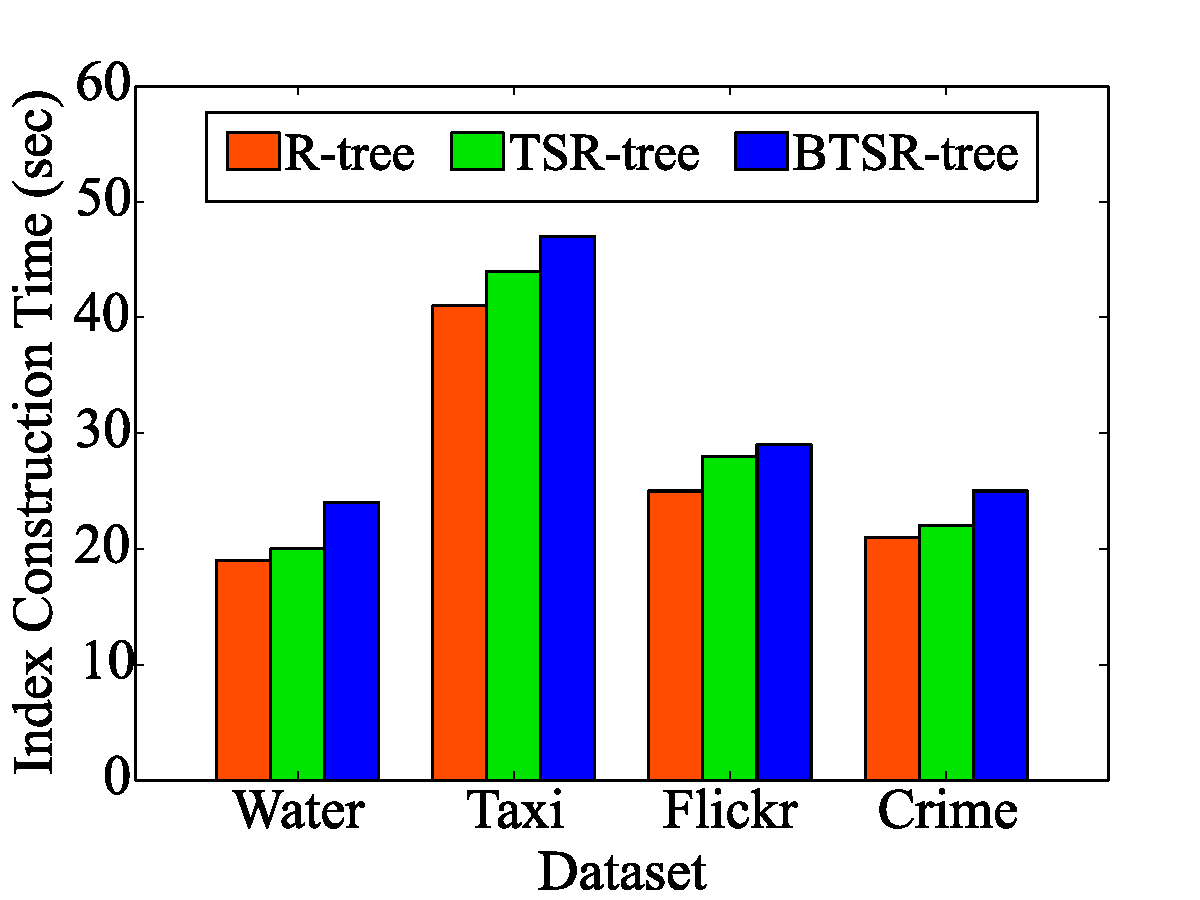
\includegraphics[width=0.23\textwidth]{figures/plots/index_time.pdf}\label{subfig:index_time}}
 \subfloat[Index size]{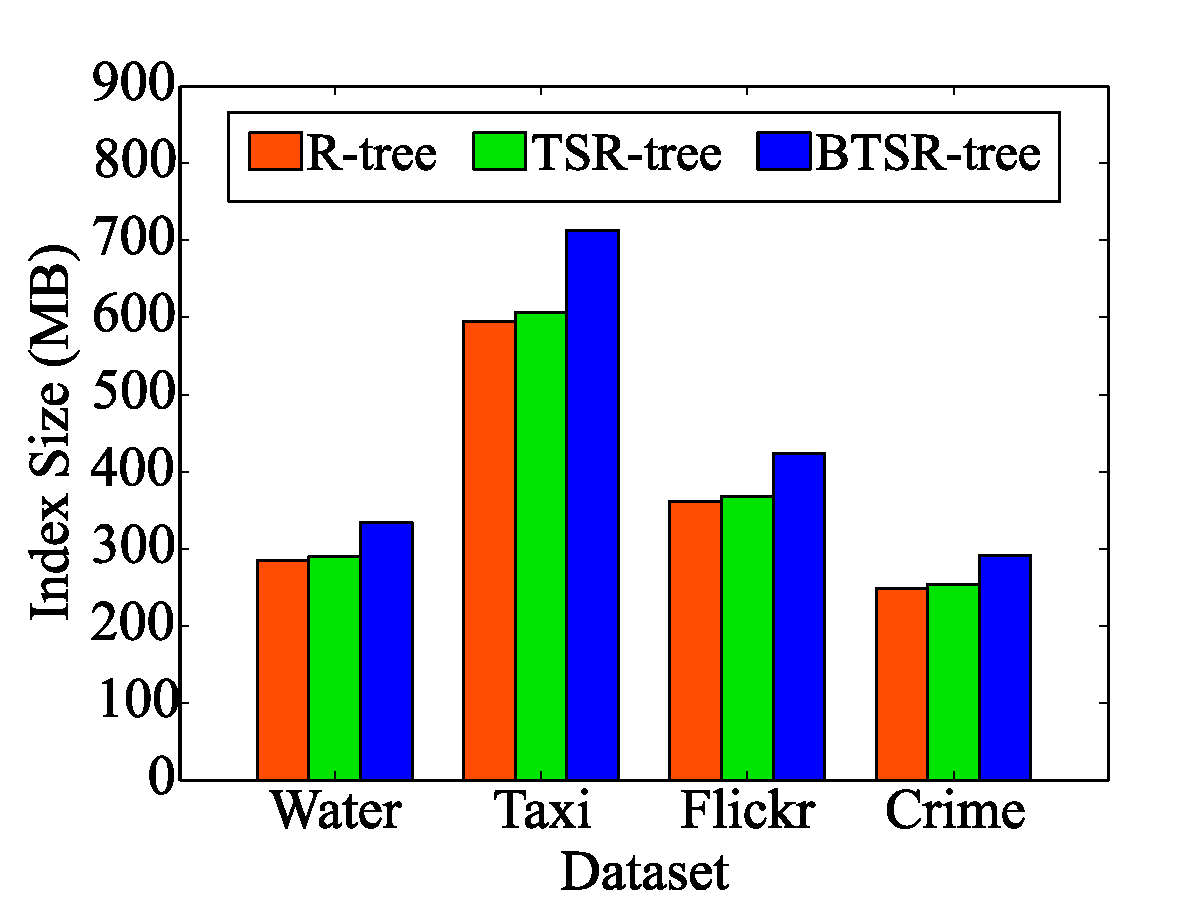
\includegraphics[width=0.23\textwidth]{figures/plots/index_size.pdf}\label{subfig:index_size}}
 \caption{Comparison of index construction time and size for each dataset.}
 \label{fig:index_construction}
\end{figure}


\begin{figure*}[t]
 \centering
 \subfloat[Water]{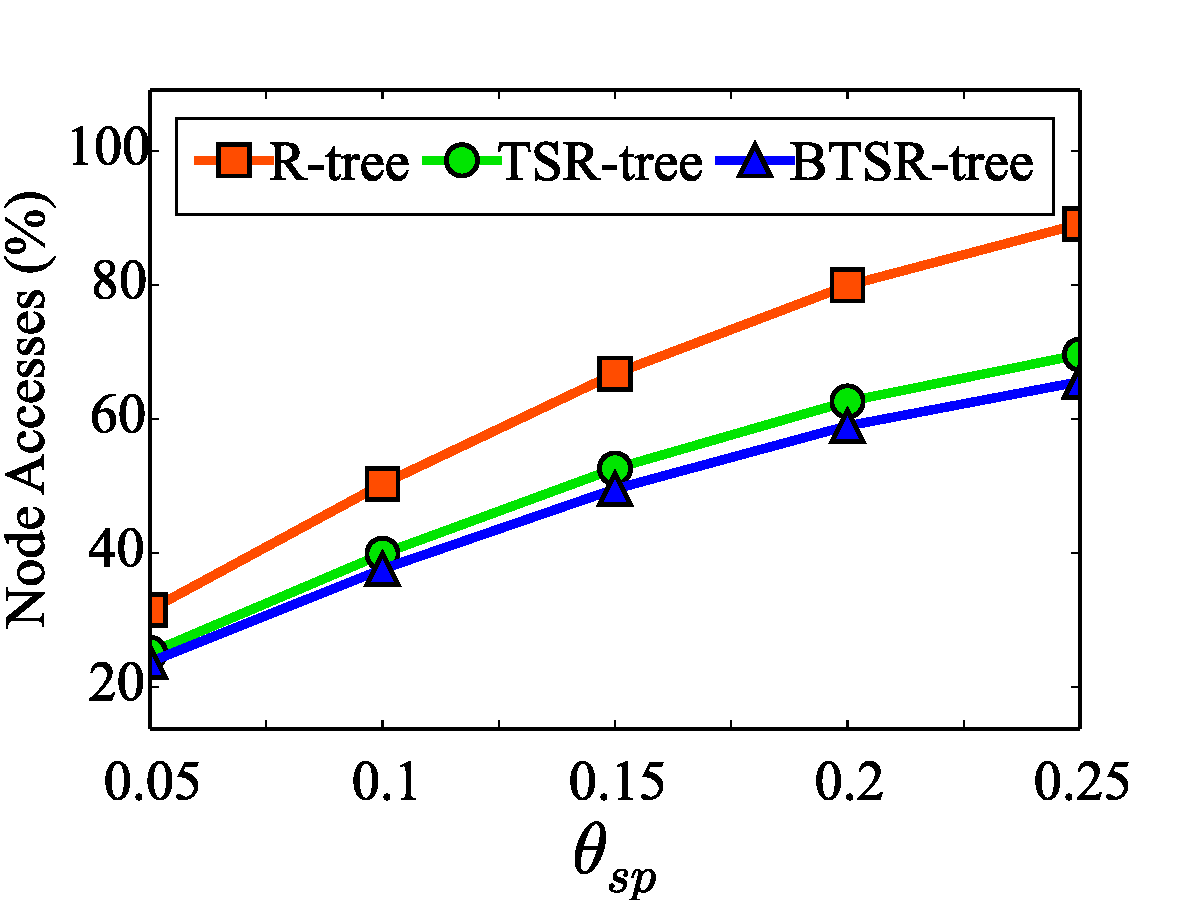
\includegraphics[width=0.246\textwidth]{figures/plots/water/qbb_theta_sp.pdf}\label{subfig:qbb_theta_sp_water}}
 \subfloat[Taxi]{\includegraphics[width=0.246\textwidth]{figures/plots/taxi/qbb_theta_sp.pdf}\label{subfig:qbb_theta_sp_taxi}}
 \subfloat[Flickr]{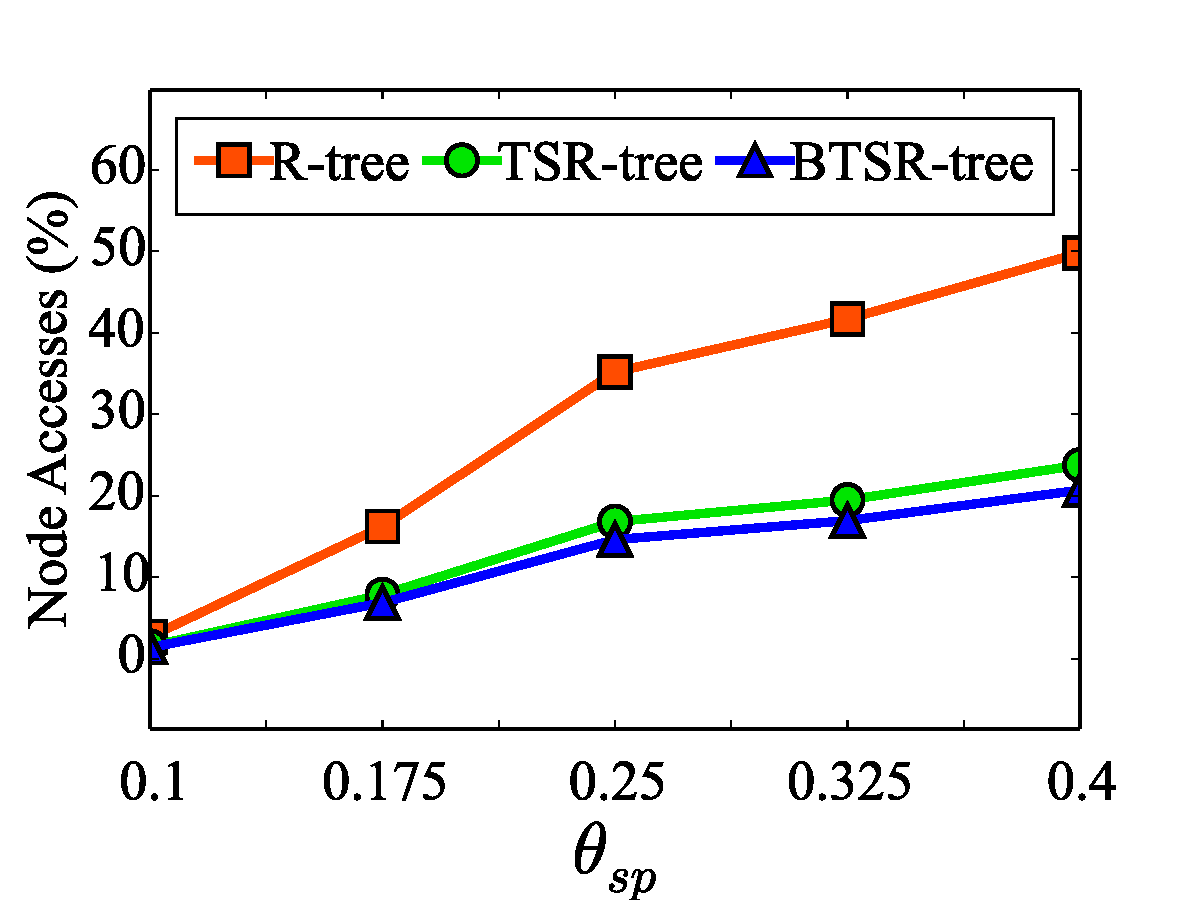
\includegraphics[width=0.246\textwidth]{figures/plots/flickr/qbb_theta_sp.pdf}\label{subfig:qbb_theta_sp_flickr}}
 \subfloat[Crime]{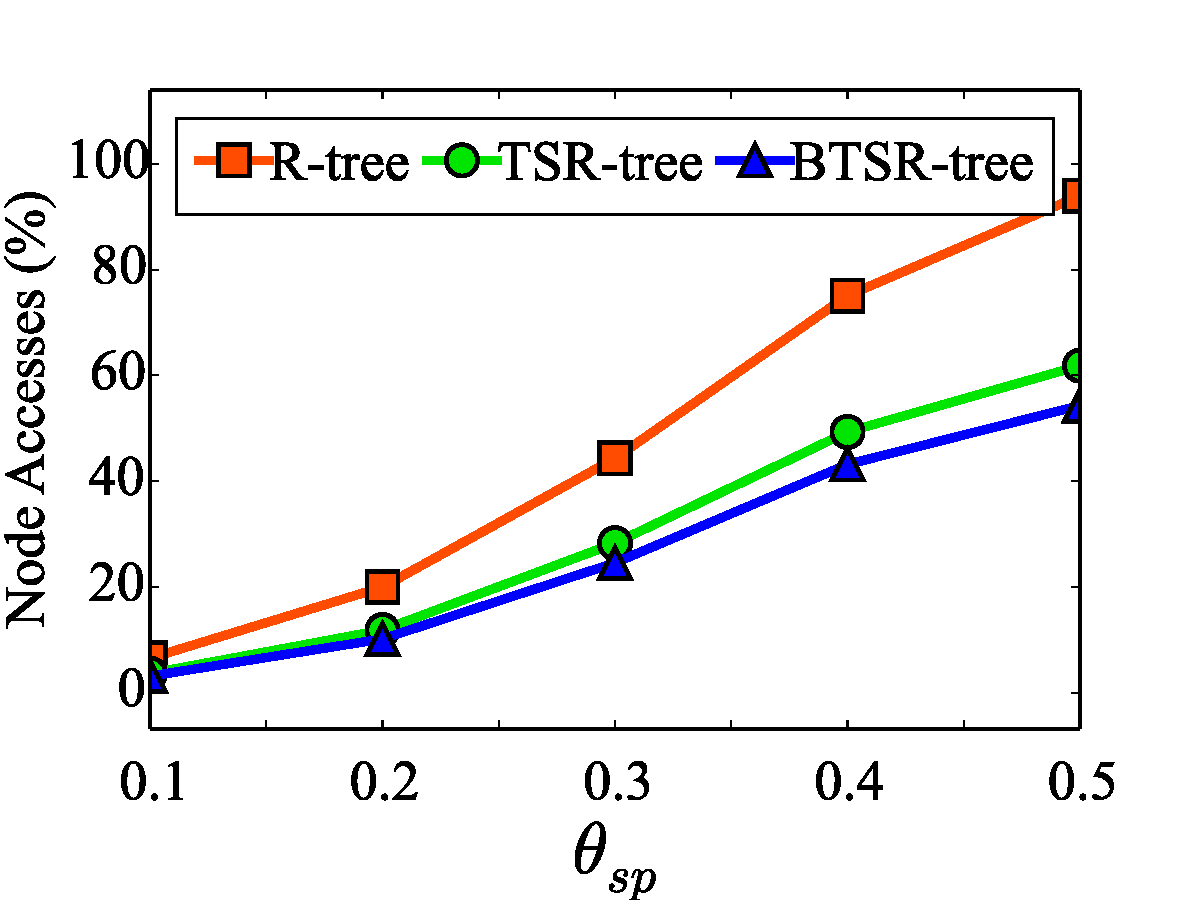
\includegraphics[width=0.246\textwidth]{figures/plots/crime/qbb_theta_sp.pdf}\label{subfig:qbb_theta_sp_crime}}
 \caption{Query $Q_{bb}(T_q, \theta_{sp}, \theta_{ts})$ with varying spatial distance threshold $\theta_{sp}$.}
 \label{fig:query_qbb_theta_sp}
\end{figure*}


\begin{figure*}[t]
 \centering
 \subfloat[Water]{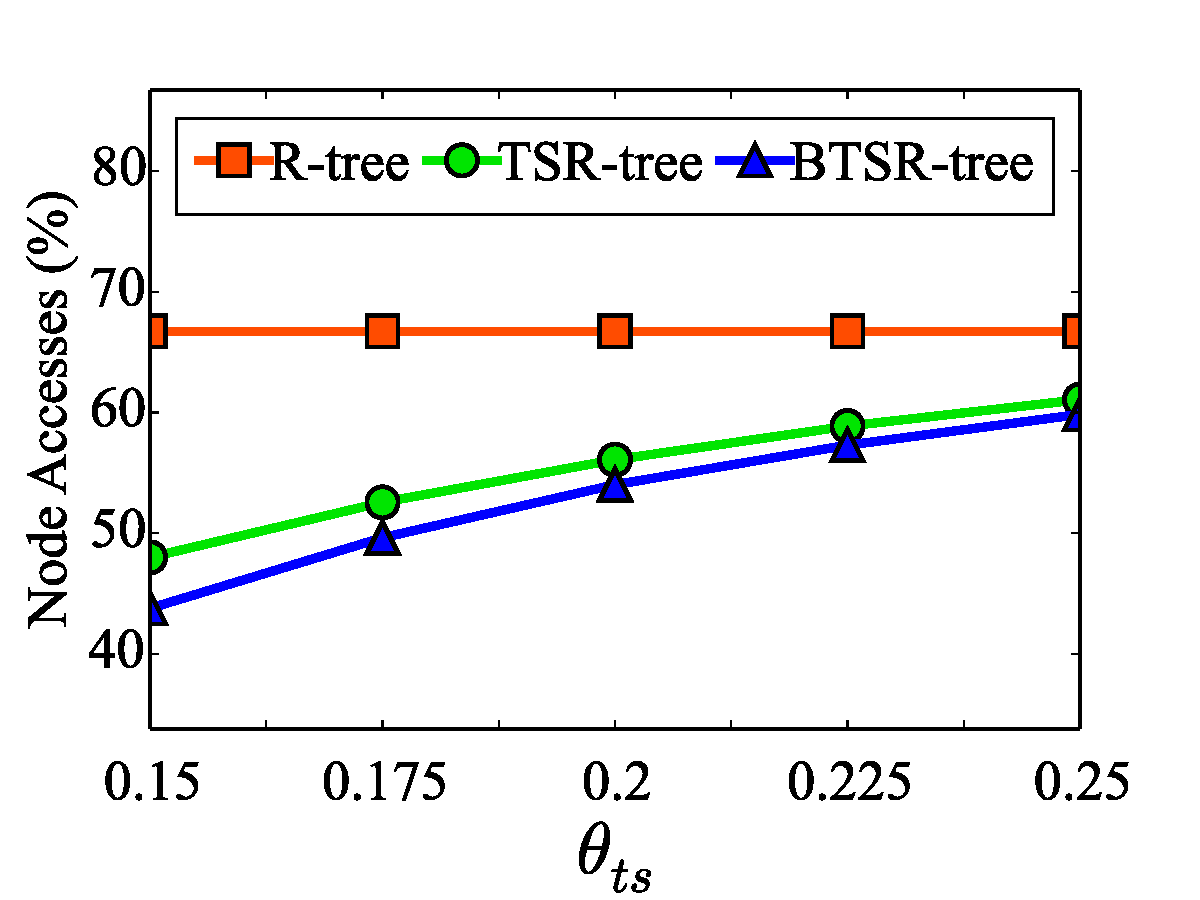
\includegraphics[width=0.246\textwidth]{figures/plots/water/qbb_theta_ts.pdf}\label{subfig:qbb_theta_ts_water}}
 \subfloat[Taxi]{\includegraphics[width=0.246\textwidth]{figures/plots/taxi/qbb_theta_ts.pdf}\label{subfig:qbb_theta_ts_taxi}}
 \subfloat[Flickr]{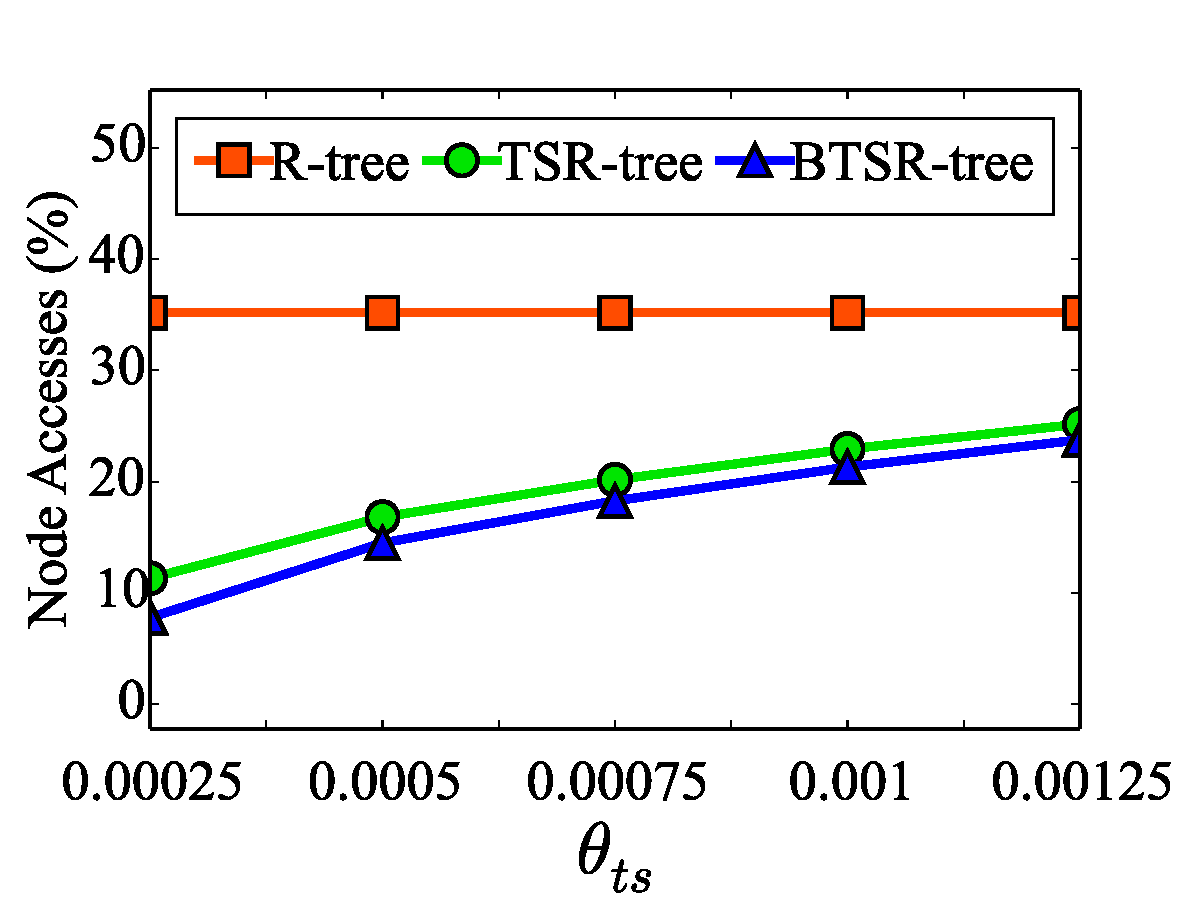
\includegraphics[width=0.246\textwidth]{figures/plots/flickr/qbb_theta_ts.pdf}\label{subfig:qbb_theta_ts_flickr}}
 \subfloat[Crime]{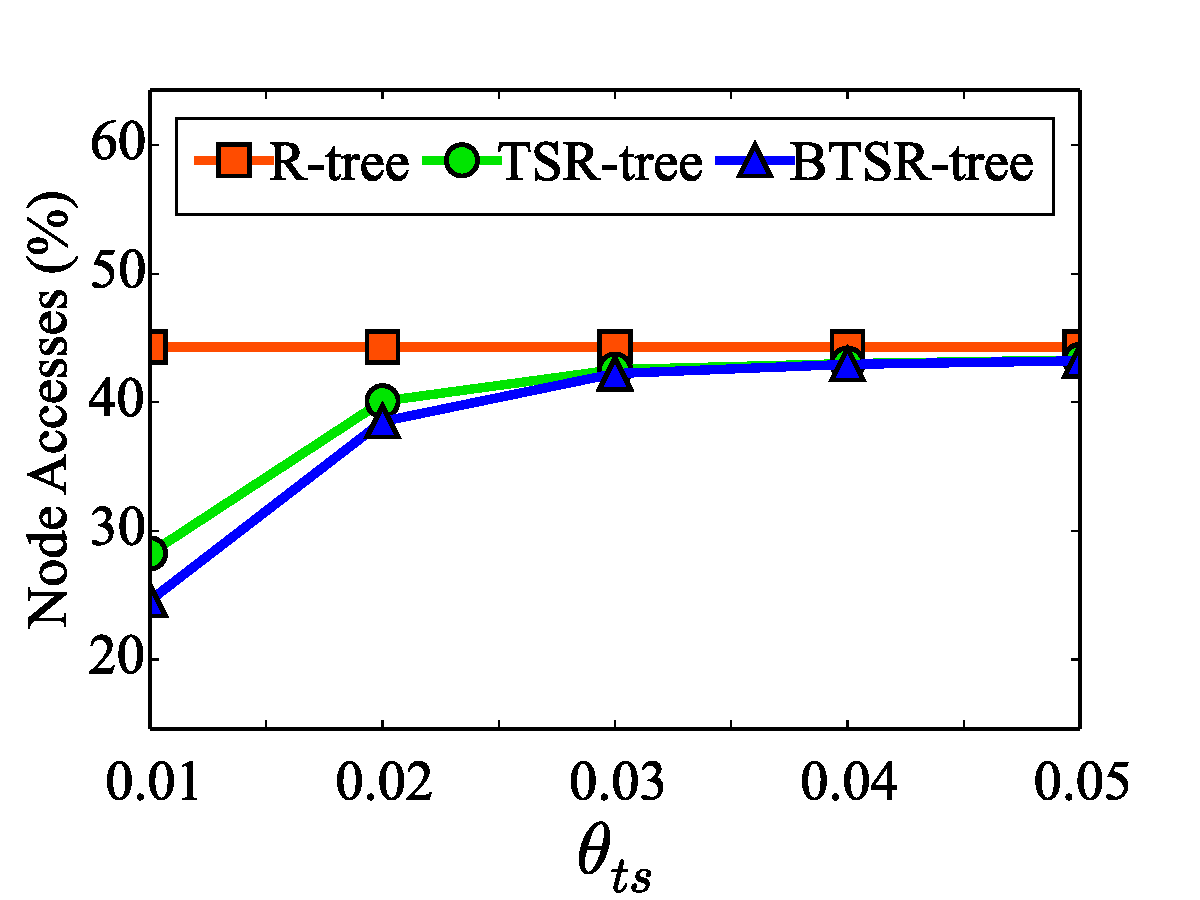
\includegraphics[width=0.246\textwidth]{figures/plots/crime/qbb_theta_ts.pdf}\label{subfig:qbb_theta_ts_crime}}
 \caption{Query $Q_{bb}(T_q, \theta_{sp}, \theta_{ts})$ with varying time series distance threshold $\theta_{ts}$.}
 \label{fig:query_qbb_theta_ts}
\end{figure*}


\begin{figure*}[t]
 \centering
 \subfloat[Water]{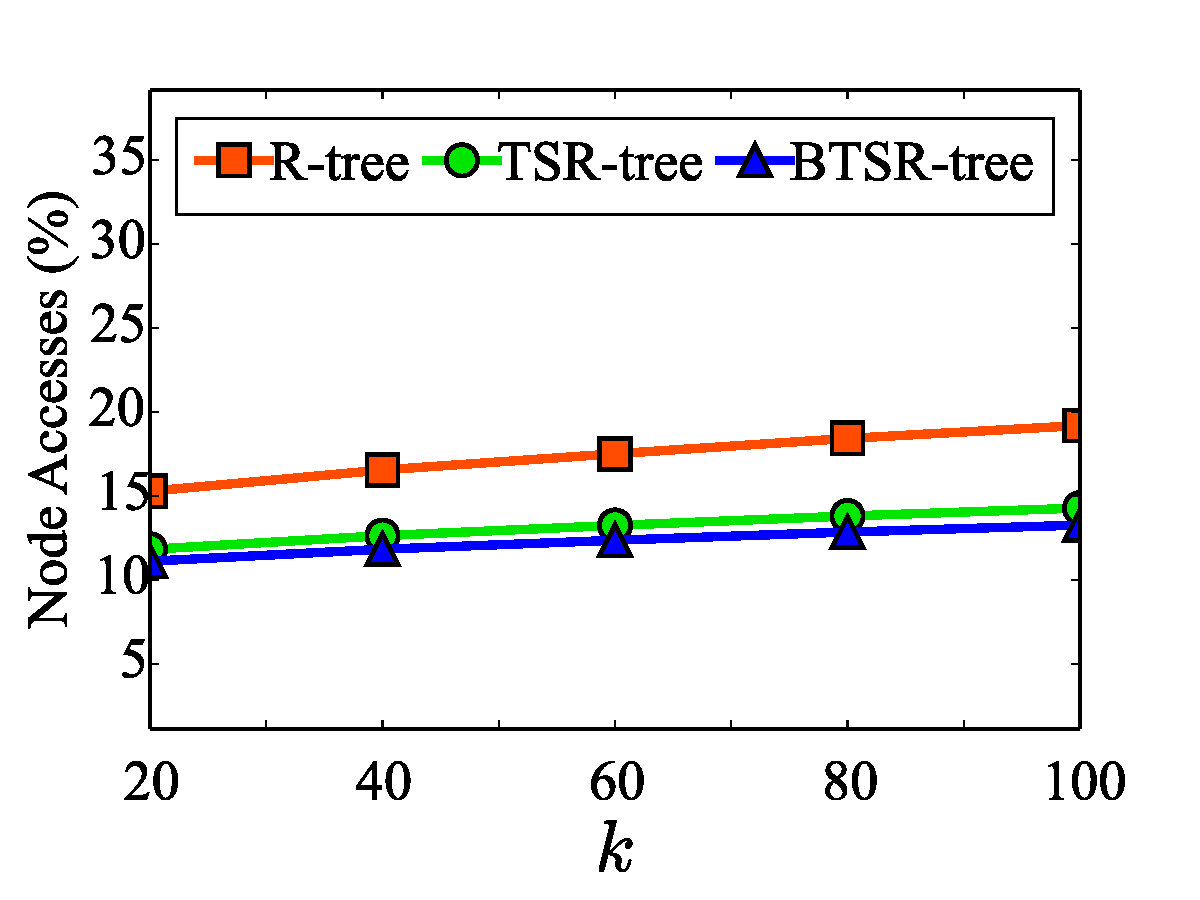
\includegraphics[width=0.246\textwidth]{figures/plots/water/qkb_k.pdf}\label{subfig:qkb_k_water}}
 \subfloat[Taxi]{\includegraphics[width=0.246\textwidth]{figures/plots/taxi/qkb_k.pdf}\label{subfig:qkb_k_taxi}}
 \subfloat[Flickr]{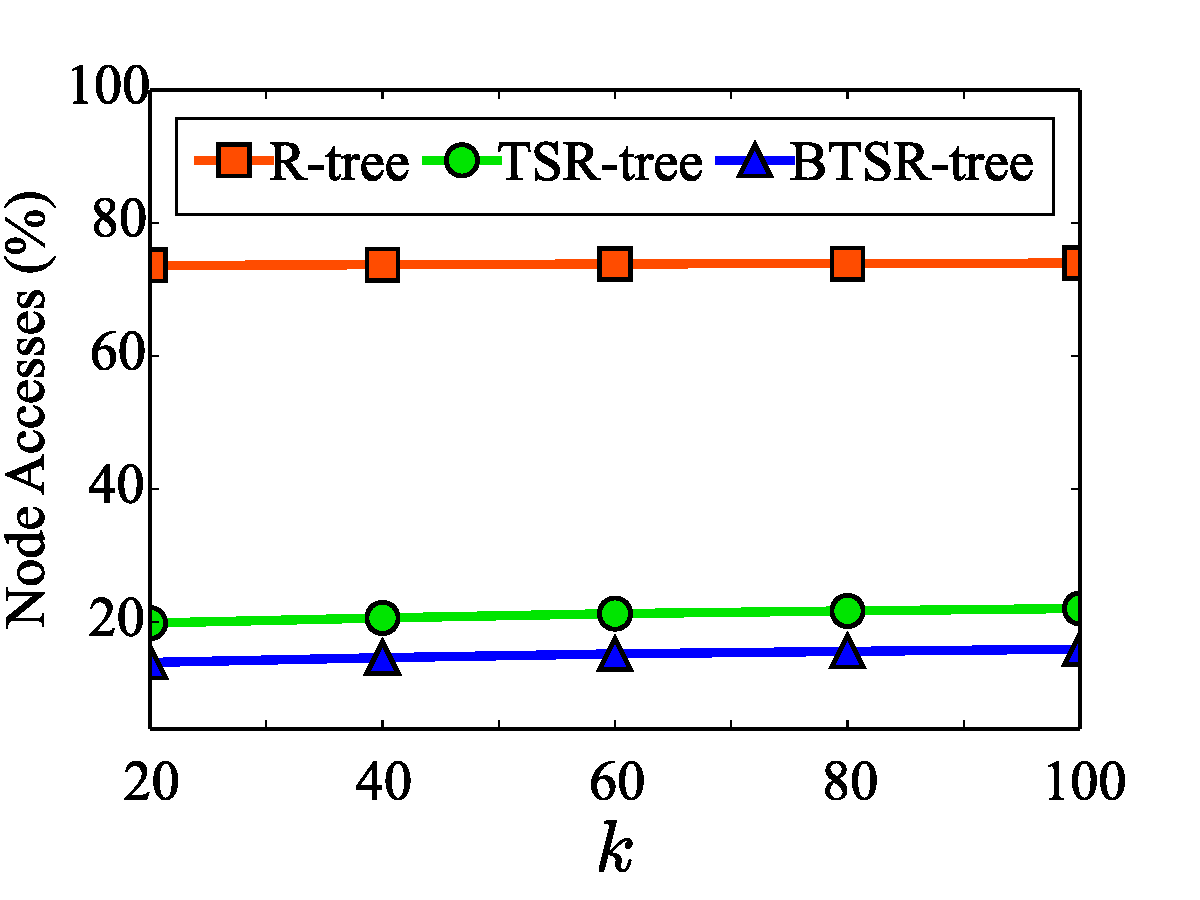
\includegraphics[width=0.246\textwidth]{figures/plots/flickr/qkb_k.pdf}\label{subfig:qkb_k_flickr}}
 \subfloat[Crime]{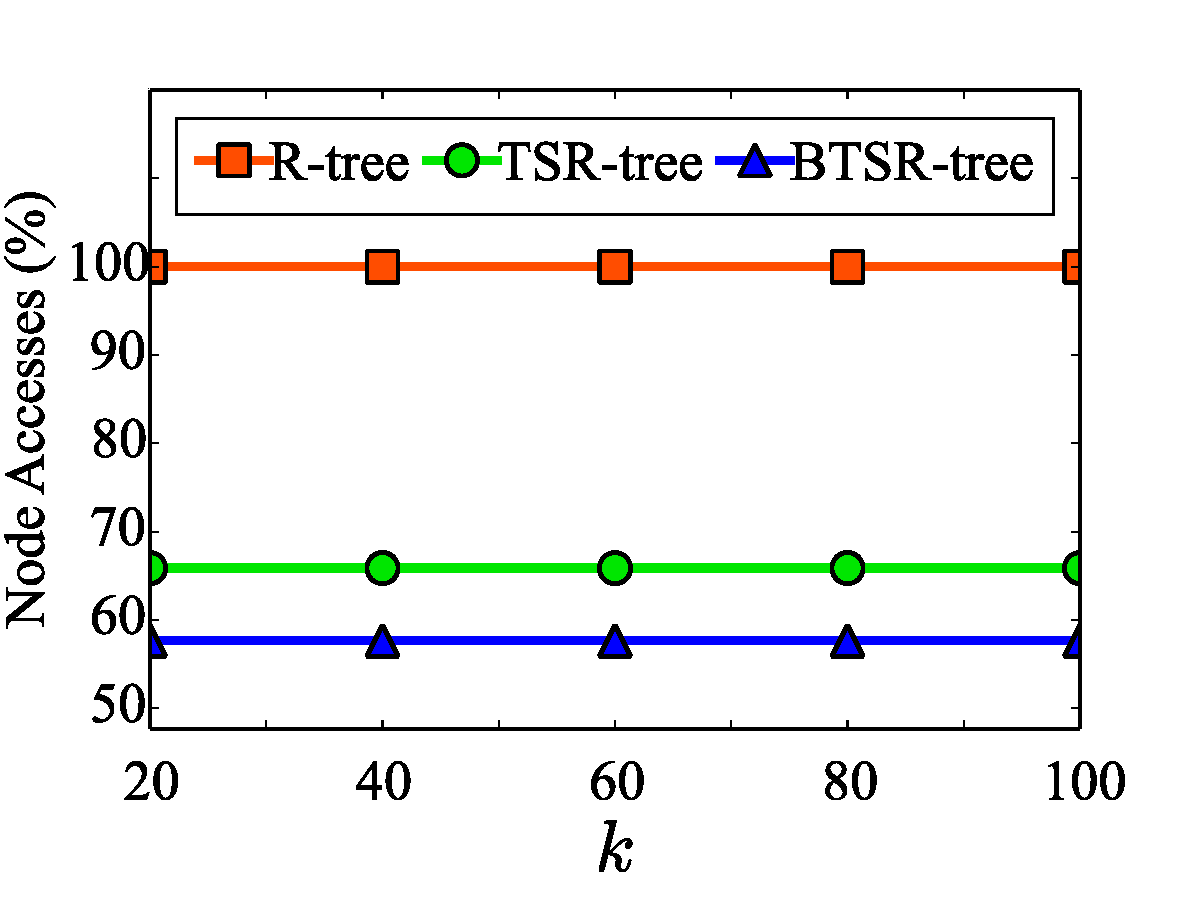
\includegraphics[width=0.246\textwidth]{figures/plots/crime/qkb_k.pdf}\label{subfig:qkb_k_crime}}
 \caption{Query $Q_{kb}(T_q, k, \theta_{ts})$ with varying number $k$ of results.}
 \label{fig:query_qkb_k}
\end{figure*}


\begin{figure*}[t]
	\centering
	\subfloat[Water]{\includegraphics[width=0.246\textwidth]{figures/plots/water/qkb_theta_ts.pdf}\label{subfig:qkb_theta_ts_water}}
	\subfloat[Taxi]{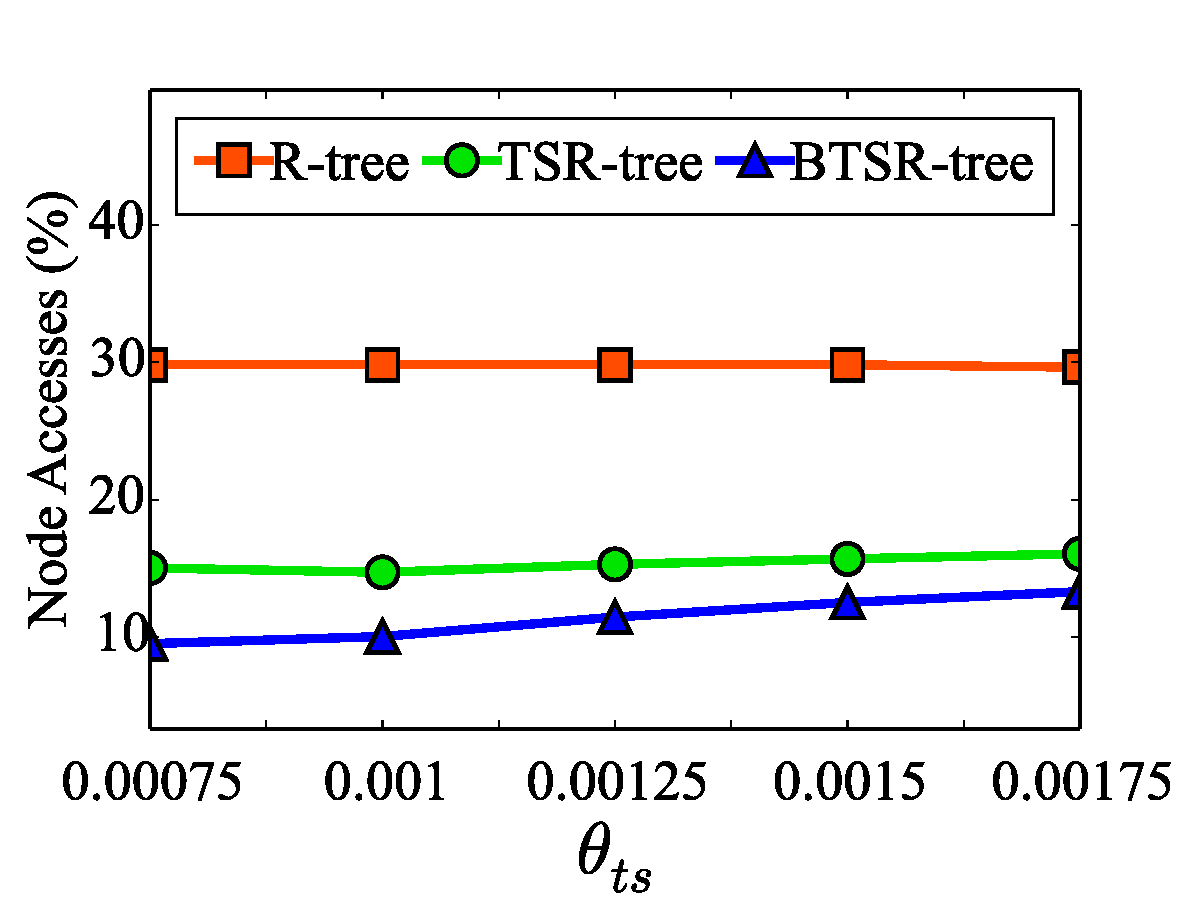
\includegraphics[width=0.246\textwidth]{figures/plots/taxi/qkb_theta_ts.pdf}\label{subfig:qkb_theta_ts_taxi}}
	\subfloat[Flickr]{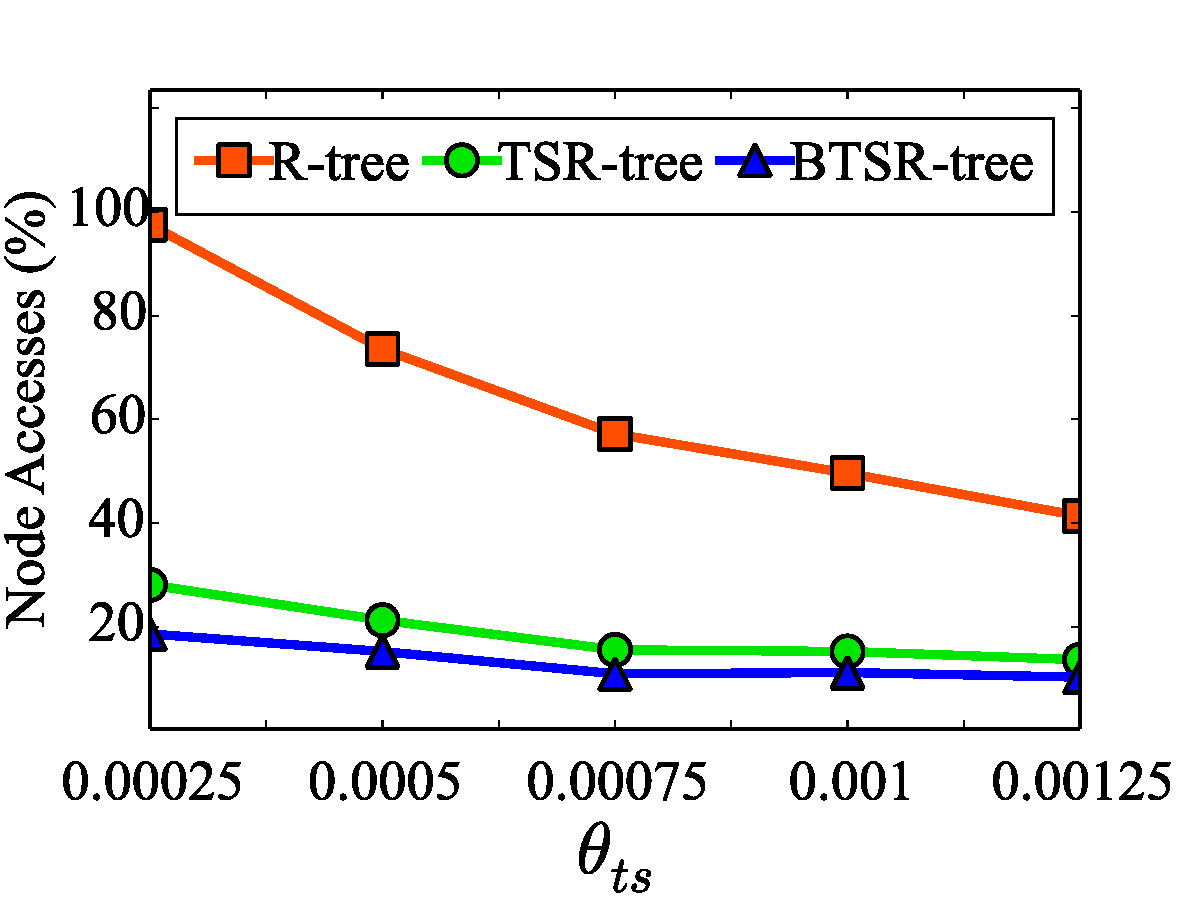
\includegraphics[width=0.246\textwidth]{figures/plots/flickr/qkb_theta_ts.pdf}\label{subfig:qkb_theta_ts_flickr}}
	\subfloat[Crime]{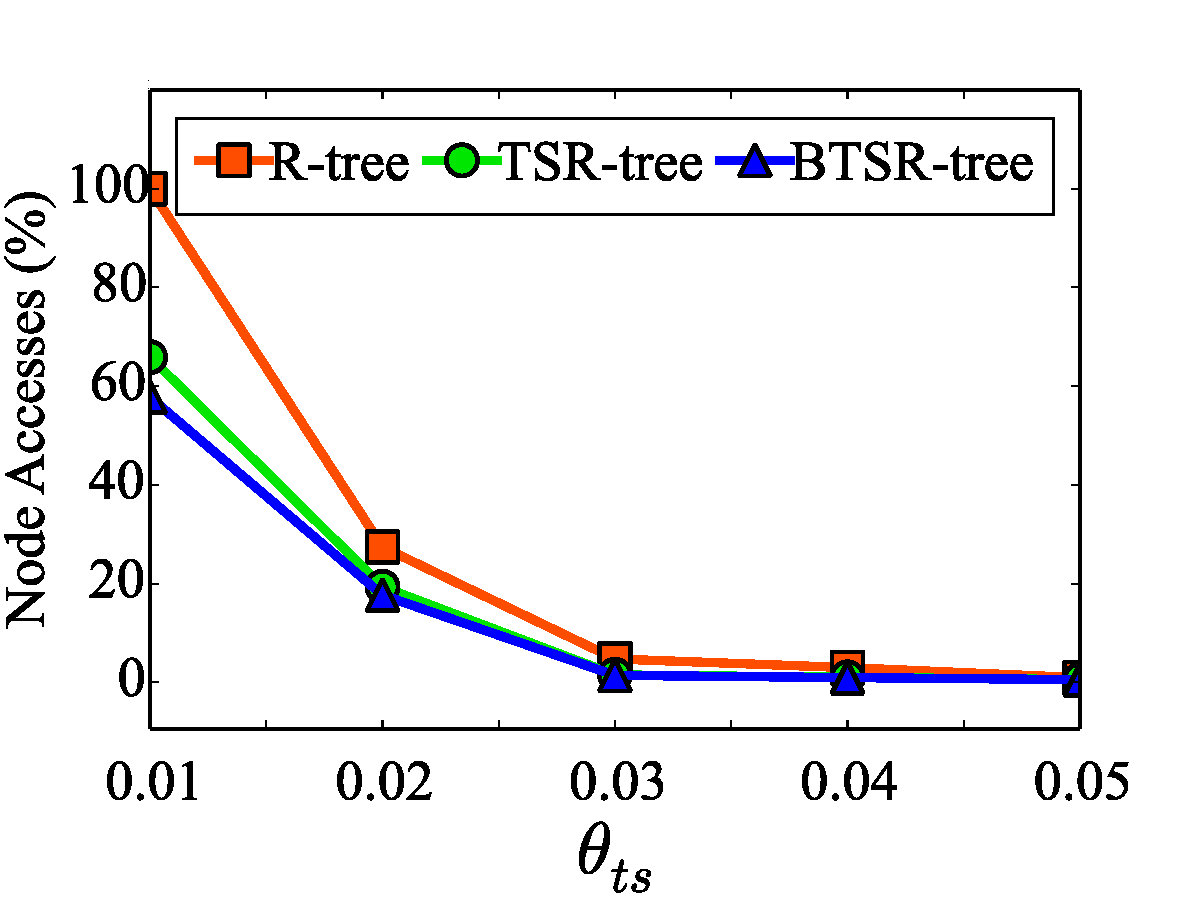
\includegraphics[width=0.246\textwidth]{figures/plots/crime/qkb_theta_ts.pdf}\label{subfig:qkb_theta_ts_crime}}
	\caption{Query $Q_{kb}(T_q, k, \theta_{ts})$ with varying time series distance threshold $\theta_{ts}$.}
	\label{fig:query_qkb_theta_ts}
\end{figure*}


\begin{figure*}[t]
	\centering
	\subfloat[Water]{\includegraphics[width=0.246\textwidth]{figures/plots/water/qbk_k.pdf}\label{subfig:qbk_k_water}}
	\subfloat[Taxi]{\includegraphics[width=0.246\textwidth]{figures/plots/taxi/qbk_k.pdf}\label{subfig:qbk_k_taxi}}
	\subfloat[Flickr]{\includegraphics[width=0.246\textwidth]{figures/plots/flickr/qbk_k.pdf}\label{subfig:qbk_k_flickr}}
	\subfloat[Crime]{\includegraphics[width=0.246\textwidth]{figures/plots/crime/qbk_k.pdf}\label{subfig:qbk_k_crime}}
	\caption{Query $Q_{bk}(T_q, \theta_{sp}, k)$ with varying number $k$ of results.}
	\label{fig:query_qbk_k}
\end{figure*}


\begin{figure*}[t]
	\centering
	\subfloat[Water]{\includegraphics[width=0.246\textwidth]{figures/plots/water/qbk_theta_sp.pdf}\label{subfig:qbk_theta_sp_water}}
	\subfloat[Taxi]{\includegraphics[width=0.246\textwidth]{figures/plots/taxi/qbk_theta_sp.pdf}\label{subfig:qbk_theta_sp_taxi}}
	\subfloat[Flickr]{\includegraphics[width=0.246\textwidth]{figures/plots/flickr/qbk_theta_sp.pdf}\label{subfig:qbk_theta_sp_flickr}}
	\subfloat[Crime]{\includegraphics[width=0.246\textwidth]{figures/plots/crime/qbk_theta_sp.pdf}\label{subfig:qbk_theta_sp_crime}}
	\caption{Query $Q_{bk}(T_q, \theta_{sp}, k)$ with varying spatial distance threshold $\theta_{sp}$.}
	\label{fig:query_qbk_theta_sp}
\end{figure*}


\begin{figure*}[t]
	\centering
	\subfloat[Water]{\includegraphics[width=0.246\textwidth]{figures/plots/water/qhb_theta_h.pdf}\label{subfig:qhb_theta_h_water}}
	\subfloat[Taxi]{\includegraphics[width=0.246\textwidth]{figures/plots/taxi/qhb_theta_h.pdf}\label{subfig:qhb_theta_h_taxi}}
	\subfloat[Flickr]{\includegraphics[width=0.246\textwidth]{figures/plots/flickr/qhb_theta_h.pdf}\label{subfig:qhb_theta_h_flickr}}
	\subfloat[Crime]{\includegraphics[width=0.246\textwidth]{figures/plots/crime/qhb_theta_h.pdf}\label{subfig:qhb_theta_h_crime}}
	\caption{Query $Q_{hb}(T_q, \theta_h, \gamma)$ with varying hybrid distance threshold $\theta_h$.}
	\label{fig:query_qhb_theta_h}
\end{figure*}


\begin{figure*}[t]
	\centering
	\subfloat[Water]{\includegraphics[width=0.246\textwidth]{figures/plots/water/qhk_k.pdf}\label{subfig:qhk_k_water}}
	\subfloat[Taxi]{\includegraphics[width=0.246\textwidth]{figures/plots/taxi/qhk_k.pdf}\label{subfig:qhk_k_taxi}}
	\subfloat[Flickr]{\includegraphics[width=0.246\textwidth]{figures/plots/flickr/qhk_k.pdf}\label{subfig:qhk_k_flickr}}
	\subfloat[Crime]{\includegraphics[width=0.246\textwidth]{figures/plots/crime/qhk_k.pdf}\label{subfig:qhk_k_crime}}
	\caption{Query $Q_{hk}(T_q, k, \gamma)$ with varying number $k$ of results.}
	\label{fig:query_qhk_k}
\end{figure*}


\subsubsection{Index Construction Time and Size}

Figure \ref{fig:index_construction} shows the index construction time and the resulting index size (i.e., memory footprint) for each dataset. Construction time of the \tsr index is slightly higher than that of the R-tree, and the same holds for the index size. This is natural, because after building the spatial part of the index, it has to be traversed in order to calculate the MBTS of each node, which incurs additional cost both for computing and for storing it in each node. Compared to the \tsr, building the \ctsr index is even more costly, since it incurs an additional time and space overhead to compute the time series bundles in each node and maintain the MBTS of each bundle. Still, these costs are not considered significant. Even for the largest dataset (Taxi), which contains $417,960$ time series and has an original size of $153$ MB, the index construction time is around $43$ seconds for \tsr and $45$ seconds for \ctsr, while the index size is around $610$ MB and $710$ MB, respectively. Note that the extra space for the \ctsr is needed for storing the bounds for each of the progressively multiple bundles in internal nodes.

%of the 5 bundles per node.

\subsubsection{Query Performance}

We compare the percentage of nodes accessed by each index in each query. All measurements are average cost per query in each particular workload.

\subsubsubsection{$Q_{bb}$}
Figure \ref{fig:query_qbb_theta_sp} illustrates the performance of the $Q_{bb}$ query on each dataset for varying spatial distance threshold ($\theta_{sp}$). Both the \tsr and the \ctsr clearly outperform the standard R-tree in all datasets, with gains in performance increasing even further as the threshold $\theta_{sp}$ increases. The standard R-tree needs to access a significant amount of nodes as it can only prune in the spatial domain. As a result, it performs increasingly worse than the \tsr and the \ctsr. Due to its tighter bounds, the \ctsr manages to prune more nodes than the \tsr, especially for larger spatial threshold values. 

Obviously, increasing the time series threshold (Figure \ref{fig:query_qbb_theta_ts}) has absolutely no impact on the performance of the standard R-tree. On the contrary, the node accesses required by the \tsr and the \ctsr are much lower. Nevertheless, these also increase with more relaxed $\theta_{ts}$, asymptotically reaching those of the R-tree. Performance of the \ctsr is better for lower values of $\theta_{ts}$, as it allows more pruning thanks to the tighter bounds of bundles. It is apparent that the sensitivity of the threshold heavily depends on the dataset. Even slightly increasing $\theta_{ts}$ in the Taxi and Flickr datasets (Figure \ref{subfig:qbb_theta_ts_taxi} and \ref{subfig:qbb_theta_ts_flickr}), significantly affects performance of both the \tsr and the \ctsr, as they are more sparse than the Water and Crime datasets (Figure \ref{subfig:qbb_theta_ts_water} and \ref{subfig:qbb_theta_ts_crime}), with a large number of time series having many zero values. Consequently, even a small increase in this threshold causes a larger amount of nodes to be probed.

\subsubsubsection{$Q_{kb}$}
Performance of $Q_{kb}$ for varying number $k$ of results is depicted in Figure \ref{fig:query_qkb_k}.  In all cases, both the \tsr and the \ctsr cope better compared to the standard R-tree. Varying the number $k$  of results does not significantly affect performance, as nearby elements tend to have similar time series values and all required results are found in close distance. This is an interesting insight, especially for the Water dataset, which suggests that neighboring households tend to have similar water consumption. The R-tree performs really poor in the Crime dataset (Figure \ref{subfig:qkb_k_crime}), requiring a full traversal ($100\%$ of its nodes), as the sought number of results cannot be found. This is not the case with the \tsr and the \ctsr, respectively accessing $65\%$ and $58\%$ of their nodes due to their effective pruning in the time series domain. 






Increasing the time series threshold $\theta_{ts}$ (Figure \ref{fig:query_qkb_theta_ts}) in $Q_{kb}$, improves performance of the R-tree and it is sometimes competitive to that of the \tsr and the \ctsr, as more nearby elements qualify as results and are thus quickly found. However, this is strongly influenced by dataset characteristics. For the Taxi dataset (Figure \ref{subfig:qkb_theta_ts_taxi}), node accesses in the R-tree are similar for different values of $\theta_{ts}$, but performance for the \ctsr slightly decreases with higher threshold values. Indeed, relaxing this threshold effectively allows more tolerance in the similarity of time series and thus, extra nodes need to be visited for checking. %This effect is also slightly visible for the Water dataset (Figure \ref{subfig:qkb_theta_ts_water}).

%\vspace{0.5mm}

\subsubsection{$Q_{bk}$}
Varying the number $k$ of results in the $Q_{bk}$ query (Figure \ref{fig:query_qbk_k}), shows similar behavior to the $Q_{kb}$ query. Similar time series are located close to each other, so $k$ results are quickly obtained once the first qualifying time series is retrieved. The R-tree is always significantly outperformed by the \tsr and \ctsr;  the effect is less apparent in the Crime dataset (Figure \ref{subfig:qbk_k_crime}).


Figure \ref{fig:query_qbk_theta_sp} illustrates performance of the $Q_{bk}$ query for varying spatial distance threshold ($\theta_{sp}$). The significantly better performance of the \tsr and the \ctsr is also apparent here, with the difference getting more pronounced with larger thresholds (i.e., wider radii). This advantage is less manifest in the Crime dataset (Figure \ref{subfig:qbk_theta_sp_crime}) because the applied thresholds cover increasingly larger spatial areas (practically the entire dataset for $\theta_{sp} =0.5$), thus more nodes need to be examined in order to identify the $k$ results. In the Taxi dataset, the performance improvement of the \ctsr compared to the \tsr is smaller due to data sparsity, which diminishes the pruning effect of bundles in the nodes of the \ctsr.

%\vspace{1mm}

\subsubsection{$Q_{hb}$ and $Q_{hk}$}
First, note that such hybrid queries cannot be possibly applied on the R-tree at all. Regarding the $Q_{hb}$ query, Figure \ref{fig:query_qhb_theta_h} plots performance for varying hybrid distance threshold ($\theta_{hb}$). The \ctsr fares better than the \tsr in all cases. The effect is more intense with smaller $\theta_{hb}$ values, since the tighter bundles in the \ctsr allow more effective pruning. For each dataset, divergence in performance between the two indices largely depends on variance among closely located time series. For instance, taxi dropoffs exhibit similar patterns locally, so the derived bounds also tend to be similar, diminishing the pruning power of both indices as shown in Figure \ref{subfig:qhb_theta_h_taxi}. Instead, when nearby time series have many diverse patterns, the \ctsr becomes more effective by allocating them to distinct bundles and offering considerable performance gain as for the Water dataset (Figure~\ref{subfig:qhb_theta_h_water}).






%The performance boost is, again, less obvious in the Taxi dataset (Figure \ref{subfig:qhb_theta_h_taxi}). 
%This behavior is consistent throughout the experimental evaluation results, which leads us to conclude that the pruning advantage of \ctsr tends to be higher for less sparse datasets, where the variance is larger in the time series domain.

Finally, Figure \ref{fig:query_qhk_k} depicts the performance of $Q_{hk}$ for varying number $k$ of results. \ctsr always outperforms \tsr  with a margin of more than $10\%$ node accesses on average, again with the exception of the Taxi dataset (Figure \ref{subfig:qhk_k_taxi}), as mentioned before.